\subsection{Proyección de ventas}

A partir del análisis previo sobre las ventas y los objetivos de recaudo individuales, en esta sección se realiza una estimación para anticipar los resultados financieros futuros de la empresa. Este ejercicio permite visualizar el comportamiento y crecimiento esperado del producto en el mercado, facilitando la identificación anticipada de utilidades, pérdidas, oportunidades de mejora y posibles deficiencias. La tabla \ref{proyeccion} muestra una estimación promedio de ventas mensuales y anuales para los diferentes planes disponibles.

\vspace{2mm}
\begin{minipage}{0.9\textwidth}
\centering
\captionof{table}[{Proyección ventas}]{ Proyección ventas. }
\label{proyeccion}
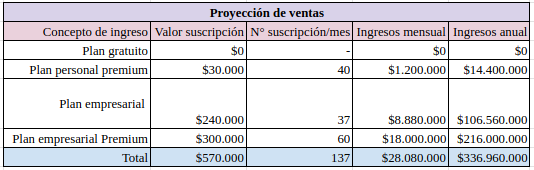
\includegraphics[width=0.6\textwidth]{Content/Images/AF/Proyeccion_de_ventas.png}
\footnote{Nota. \textup{Fuente : Autores.}}
\end{minipage}

Se toma como referencia la proyección del IPC en Colombia para los próximos cinco años, con el fin de estimar los flujos de efectivo que la empresa podría gestionar bajo el plan de negocio. La tabla \ref{ipc} presenta esta información indexada.

\vspace{2mm}
\begin{minipage}{0.9\textwidth}
\centering
\captionof{table}[{IPC}]{ IPC. }
\label{ipc}
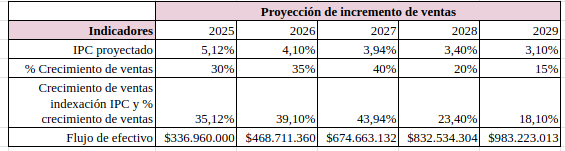
\includegraphics[width=0.6\textwidth]{Content/Images/AF/Proyeccion_de_incremento_ventas.png}
\footnote{Nota. \textup{Fuente : Autores.}}
\end{minipage}
